\documentclass[tikz]{standalone}

\usetikzlibrary{shapes,arrows,shadows,calc, angles}
\usetikzlibrary{arrows,shapes}
\usetikzlibrary{positioning}
\usetikzlibrary{patterns.meta}
\usetikzlibrary{decorations, decorations.pathreplacing}

\definecolor{fg}{rgb}{0,0,0}
\definecolor{bg}{rgb}{1,1,1}

\tikzstyle{box}=[draw, rounded corners , text width=40mm,
anchor=center,text centered,text=fg, font=\bfseries] % text width=33mm,

\tikzstyle{myarrow}=[->, >=stealth, very thick, rounded corners=2mm]
\tikzstyle{mythinarrow}=[myarrow, line width=0.25mm]

\tikzstyle{conv}=[box, fill=red!60]
\tikzstyle{norm}=[box, fill=yellow!60]
\tikzstyle{concatenation}=[box, fill=cyan!60]

\begin{document}

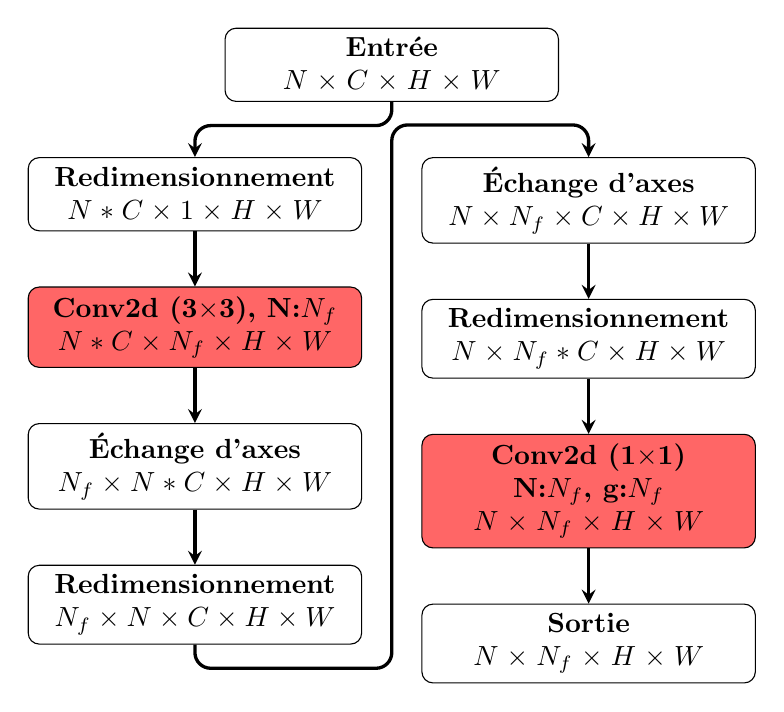
\begin{tikzpicture}[node distance=7mm]

    \node[box] (X) {Entrée\\$N \times C \times H \times W$};

    \node[box, below=of X, xshift=-25mm] (X2) {Redimensionnement $N*C \times 1 \times H \times W$} ;
    \draw[myarrow] (X.south) -- ++ (0mm, -3mm) -| (X2) ;
    

    \node[conv, below=of X2] (conv1) {Conv2d (3$\times$3), N:$N_f$\\$N*C \times N_f \times H \times W$} ;
    \draw[myarrow] (X2) -- (conv1) ;
    

    \node[box, below=of conv1] (swap1) {Échange d'axes\\$N_f \times N*C \times H \times W$} ;
    \draw[myarrow] (conv1) -- (swap1) ;

    \node[box, below=of swap1] (reshape1) {Redimensionnement\\$N_f \times N \times C \times H \times W$} ;
    \draw[myarrow] (swap1) -- (reshape1) ;

    \node[box, below=of X, xshift=25mm] (swap2) {Échange d'axes\\$N \times N_f \times C \times H \times W$} ;
    \draw[myarrow] (reshape1.south) |- ++ (25mm, -3mm) -- ++(0, 69mm) -| (swap2) ;

    \node[box, below=of swap2] (reshape2) {Redimensionnement\\$N \times N_f * C \times H \times W$} ;
    \draw[myarrow] (swap2) -- (reshape2) ;
    
    \node[conv, below=of reshape2] (conv2) {Conv2d (1$\times$1) N:$N_f$, g:$N_f$\\$N \times N_f \times H \times W$} ;
    \draw[myarrow] (reshape2) -- (conv2) ;

    \node[box, below=of conv2] (Y) {Sortie\\$N \times N_f \times H \times W$} ;
    \draw[myarrow] (conv2) -- (Y) ;
    
    % \node[norm, below=of conv3] (transition) {Transition layer ($N: N_3 // 2$)} ;
    % \draw[myarrow] (conv3) -- (transition) ;
    
    % \draw[myarrow] (conv3) -- (add) ;
    % \draw[myarrow] (X) -- ++ (0, -7mm) -| ++ (-25mm, -15mm) |- (add) ;
    
\end{tikzpicture}

\end{document}